% Uncomment this to make slides with overlays:
%\documentclass[slides]{beamer}

% Uncomment these (but comment the above \documentclass line) to make handouts:
\documentclass[handout]{beamer}

% Uncomment these to have more than one slide per page
\usepackage{pgfpages}
\pgfpagesuselayout{2 on 1}[border shrink=5mm]
\pgfpageslogicalpageoptions{1}{border code=\pgfusepath{stroke}}
\pgfpageslogicalpageoptions{2}{border code=\pgfusepath{stroke}}

\usepackage[]{graphicx, color, hyperref}

\mode<presentation>
{
	%\usetheme[secheader]{Boadilla}
	%\usecolortheme[rgb={.835, .102,.169}]{structure}  
	\usetheme[width= 0cm]{Goettingen}
	%\setbeamercovered{transparent}
}
\setbeamertemplate{navigation symbols}{}
\setbeamertemplate{footline}[frame number]

\definecolor{blue2}{rgb}{0.278,0.278,0.729} 
\newcommand{\blue}[1]{\textcolor{blue2}{#1}}
\newcommand{\white}[1]{\textcolor{white}{#1}}
\newcommand{\red}[1]{\textcolor{red}{#1}}
\newcommand{\xbar}{\overline{x}}
\newcommand{\ybar}{\overline{y}}
\newcommand{\phat}{\widehat{p}}
\newcommand{\prob}{\mbox{Pr}}
\newcommand{\E}{\mathbb{E}}
\newcommand{\Var}{\mbox{Var}}
\newcommand{\cp}{\oplus}
\newcommand{\cm}{\circleddash}


\title{Lecture 19: ANOVA Part I}
\author{Chapter 5.5}
\date{}


\begin{document}
%------------------------------------------------------------------------------
\begin{frame}
\titlepage
\end{frame}
%------------------------------------------------------------------------------


%------------------------------------------------------------------------------
\begin{frame}[fragile]
\frametitle{Discussion of Quiz}
\blue{Question 1}:  Why did $\frac{1}{20}$ studies yield a positive/significant result i.e. that there is a link between jelly beans and acne?

\vspace{0.5cm}


\pause Not that the p-value is 0.05, rather that \blue{$\alpha=0.05$}:
\pause\begin{itemize}
\item (pre-specified) significance level AKA
\item type I error rate AKA
\item false positive rate
\end{itemize}
\pause i.e. we expect 1 out of 20 results to be significant even if there is no effect by chance alone.


\end{frame}
%------------------------------------------------------------------------------


%------------------------------------------------------------------------------
\begin{frame}[fragile]
\frametitle{Publication Bias}

\begin{center}
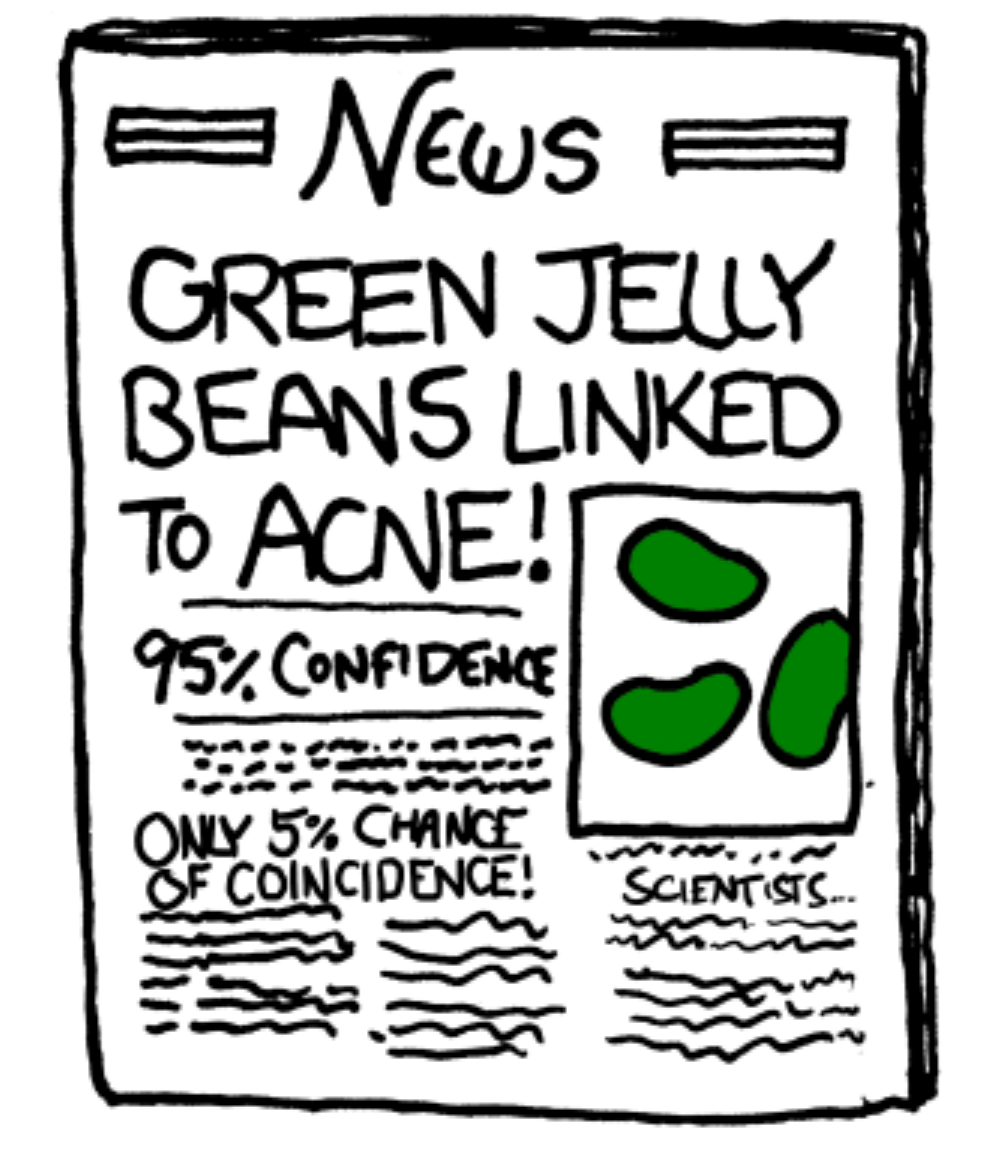
\includegraphics[width=0.5\textwidth]{figure/jelly.png}
\end{center}

\end{frame}
%------------------------------------------------------------------------------


%------------------------------------------------------------------------------
\begin{frame}[fragile]
\frametitle{Publication Bias}
\blue{Publication bias}: people only highlight significant/positive results.  \pause Wikipedia: ``occurs when the publication of research results \blue{depends on their nature and direction}.''

\vspace{0.5cm}

\pause To counter this, some medical journals like
\begin{itemize}
\item New England Journal of Medicine
\item The Lancet
\item Journal of the American Medical Association
\end{itemize}
\pause require registration of a trial \blue{before} it starts so that unfavorable results are not withheld from publication. 

\vspace{0.5cm}

\pause Journal of \blue{Negative Results}:  \blue{\url{http://www.jnrbm.com/}}

\end{frame}
%------------------------------------------------------------------------------


%------------------------------------------------------------------------------
\begin{frame}[fragile]
\frametitle{Publication Bias}

\begin{center}
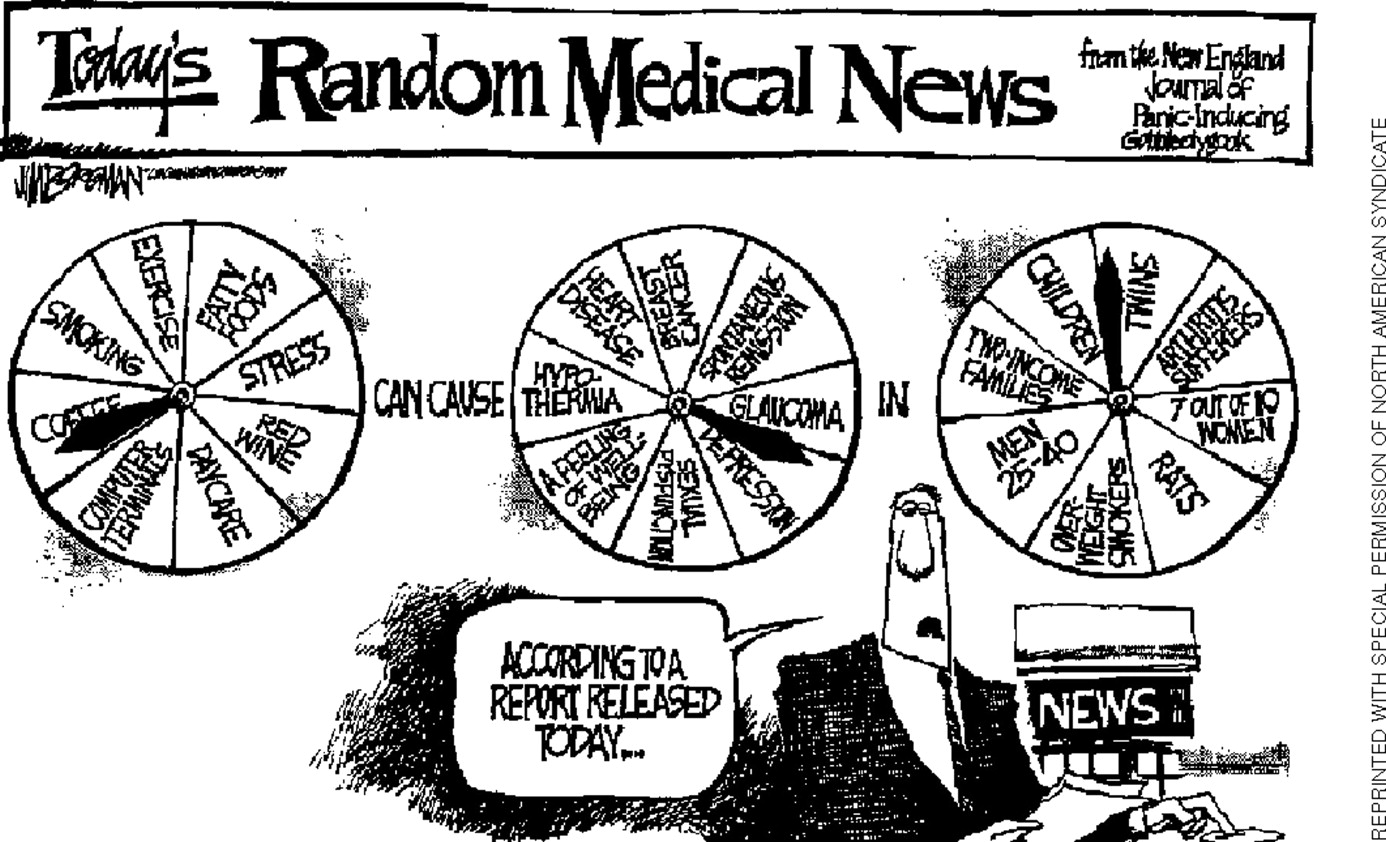
\includegraphics[width=\textwidth]{figure/wheel.jpg}
\end{center}
\end{frame}
%------------------------------------------------------------------------------


%%------------------------------------------------------------------------------
%\begin{frame}[fragile]
%\frametitle{What $\alpha$ to Use?}
%Should I use $\alpha=0.05$ as my significance level?  Before using it, put some thought into the balance between:
%\begin{itemize}
%\pause \item \blue{Type I errors}.  Setting a smaller $\alpha$ yields a more \blue{conservative} procedure: all things being equal, you will reject $H_0$ less often.  
%\pause \item \blue{Type II errors}.  Setting a bigger $\alpha$ yields a more \blue{liberal} procedure: all things being equal, you will reject $H_0$ more often.  
%\end{itemize}
%
%\end{frame}
%%------------------------------------------------------------------------------


%%------------------------------------------------------------------------------
%\begin{frame}[fragile]
%\frametitle{Multiple Testing}
%A related issue is the statistical concept of \blue{multiple testing}.
%
%\vspace{0.5cm}
%
%\pause Say we are conducting many experiments, and $H_0$ is true for all of them.  If you repeat experiments many times, you're bound to get a significant result eventually just by \blue{chance alone}.
%
%\end{frame}
%%------------------------------------------------------------------------------
%
%
%%------------------------------------------------------------------------------
%\begin{frame}[fragile]
%\frametitle{Multiple Testing}
%
%What do people do? Make the $\alpha$ stricter!  i.e. 
%\pause \begin{itemize}
%\item make the $\alpha$ smaller
%\item i.e. less chance the p-value is smaller than $\alpha$
%\item i.e. less chance of incorrectly rejecting $H_0$ when it is true
%\end{itemize}
%
%\vspace{0.25cm}
%
%\pause Use the \blue{Bonferroni correction} to $\alpha$:  If you are conducting $n$ tests, use $\alpha^* = \frac{\alpha}{n}$. More later...
%
%\end{frame}
%%------------------------------------------------------------------------------


%------------------------------------------------------------------------------
\begin{frame}[fragile]
\frametitle{Discussion of Quiz}
\blue{Question 2}:  Say a very successful entrepreneur named Jamie puts out an autobiography called ``How to win at life.''  In it, Jamie details a plan to "win" at the various dimensions of life.  Jamie states "I followed these steps, and look at me now!  You should do the same!"  Critique this statement keeping the comic in mind. 

\vspace{0.25cm}

\pause There might have been 9999 people who did the same things but perhaps aren't as successful.  Those people generally don't get book deals so we don't know about them.

\end{frame}
%------------------------------------------------------------------------------


%------------------------------------------------------------------------------
\begin{frame}[fragile]
\frametitle{Interpreting Confidence Intervals}

Page 180: They use the term ``we are \blue{95\% confident} that the population parameter is between \ldots''.

\begin{itemize}
\pause\item This is shorthand for ``if we repeat this procedure 100 times, then we expect 95 \ldots''
\pause\item and not ``there is a 95\% probability the CI contains the population parameter.''
\pause\item Think as ``using a procedure that is 95\% reliable, this interval is where we think the population parameter is.''
\end{itemize}

\end{frame}
%------------------------------------------------------------------------------



%%-------------------------------------------------------------------------------
%\begin{frame}
%\frametitle{Previously: Conditions for Using t Distribution}
%%
%% Comment this
%%
%We use the $t$ distribution when you have
%
%\begin{itemize}
%\pause \item $n$ is small.
%\pause \item \blue{Independence}: $n \leq 10\% $ rule
%%or if we have an experiment or random process we check that each observation were independent
%\pause \item \blue{Observations come from a nearly normal distribution}:
%\begin{itemize}
%\item Look at a histogram of the data (difficult when $n$ is small)
%\item Consider whether any previous experiences alert us that the data may be normal
%\end{itemize}
%\end{itemize}  
%	
%\end{frame}
%%-------------------------------------------------------------------------------


%%------------------------------------------------------------------------------
%\begin{frame}[fragile]
%\frametitle{Analysis of Variance (ANOVA)}
%A farmer has the choice of four tomato fertilizers and wants to compare their performance in terms of crop yield.
%\begin{center}
%\pause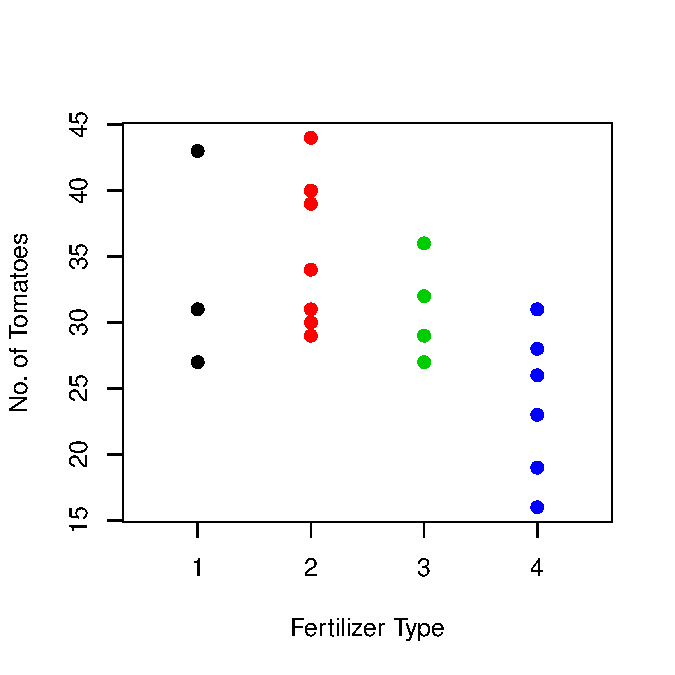
\includegraphics[width=0.65\textwidth]{figure/lec22-003}
%\end{center}
%
%\end{frame}
%%------------------------------------------------------------------------------
%
%
%%------------------------------------------------------------------------------
%\begin{frame}[fragile]
%\frametitle{Analysis of Variance (ANOVA)}
%A farmer has the choice of four tomato fertilizers and wants to compare their performance in terms of crop yield.
%\begin{center}
%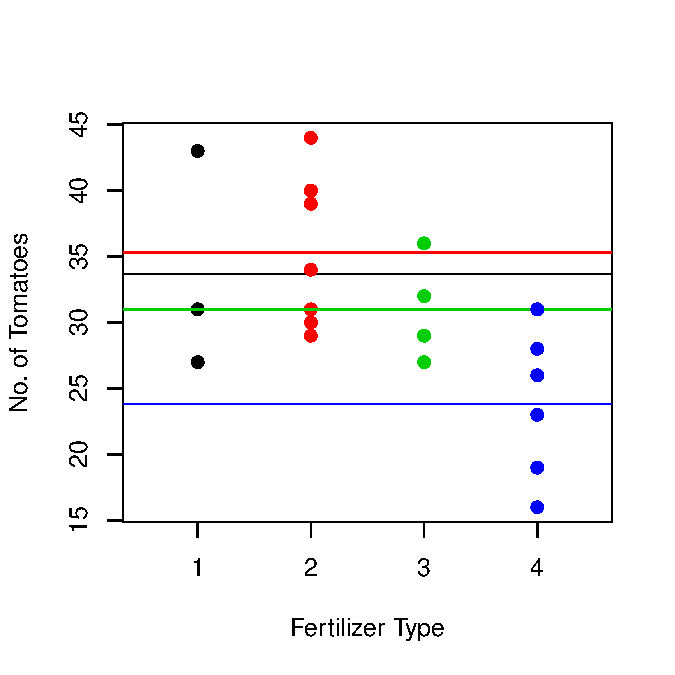
\includegraphics[width=0.65\textwidth]{figure/lec22-004}
%\end{center}
%
%\end{frame}
%%------------------------------------------------------------------------------


%------------------------------------------------------------------------------
\begin{frame}[fragile]
\frametitle{Analysis of Variance (ANOVA)}

A farmer wants to compare the performance of 4 fertilizers in terms of tomato yield.   We have $k=4$ groups AKA \blue{levels of a factor}.

\begin{itemize}
\pause\item They assign $n_i$ plants to each of the $k=4$ fertilizers:
\[
\begin{array}{cccc|c}
n_1 & n_2 & n_3 & n_4 &\mbox{total }n\\
\hline
3 & 7 & 4 & 6 & 20
\end{array}
\]
\pause\item They count the number of tomatoes on each plant
\end{itemize}

\end{frame}
%------------------------------------------------------------------------------


%-------------------------------------------------------------------------------
\begin{frame}
\frametitle{Tomato Fertilizer}
They compare the performance in terms of \# of tomatoes yielded. \textcolor{white}{Plot the sample mean of each level.} \textcolor{white}{Question: are the mean tomato yields different?}  
\setkeys{Gin}{width=0.55\textwidth}
\begin{center}
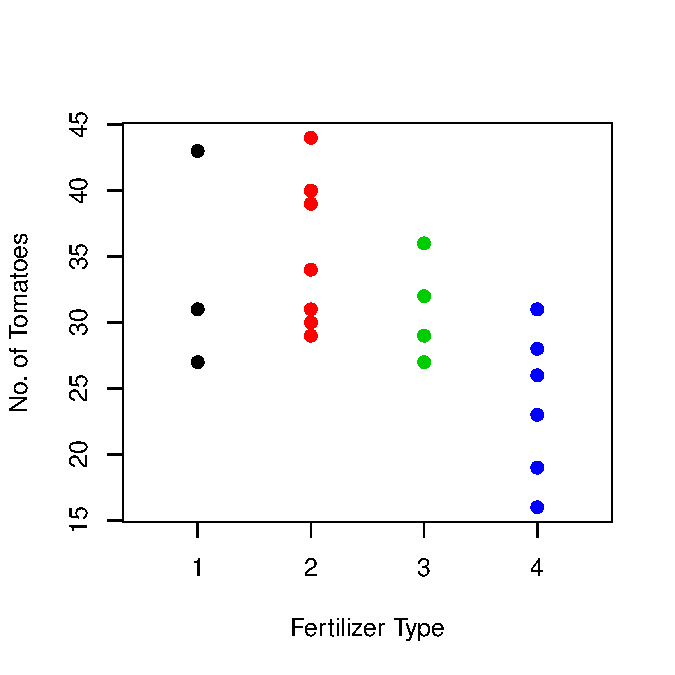
\includegraphics{figure/lec22-003}
\end{center}
\end{frame}
%-------------------------------------------------------------------------------


%-------------------------------------------------------------------------------
\addtocounter{framenumber}{-1}
\begin{frame}
\frametitle{Tomato Fertilizer}
They compare the performance in terms of \# of tomatoes yielded. Plot the sample mean of each level. \textcolor{white}{Question:  are the mean tomato yields different?} 
\setkeys{Gin}{width=0.55\textwidth}
\begin{center}
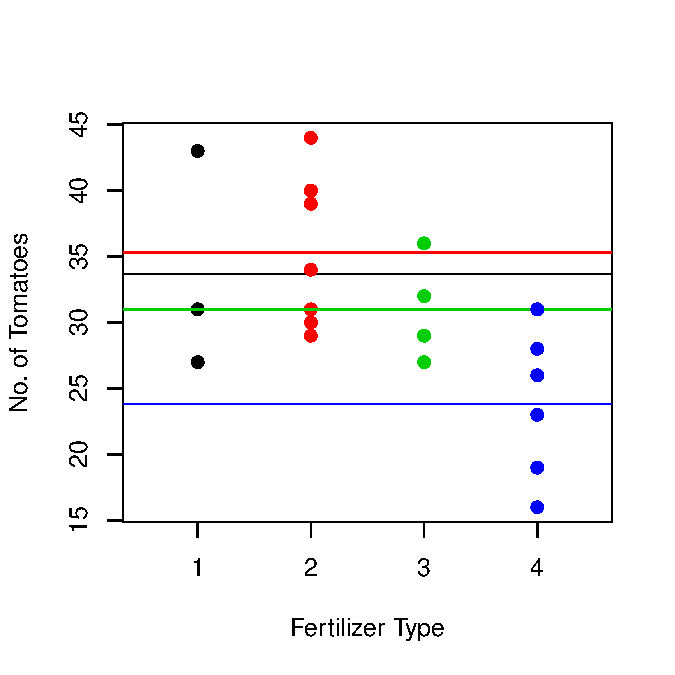
\includegraphics{figure/lec22-004}
\end{center}
\end{frame}
%-------------------------------------------------------------------------------


%-------------------------------------------------------------------------------
\addtocounter{framenumber}{-1}
\begin{frame}
\frametitle{Tomato Fertilizer}
They compare the performance in terms of \# of tomatoes yielded. Plot the sample mean of each level. \blue{Question:  are the mean tomato yields different?}
\setkeys{Gin}{width=0.55\textwidth}
\begin{center}
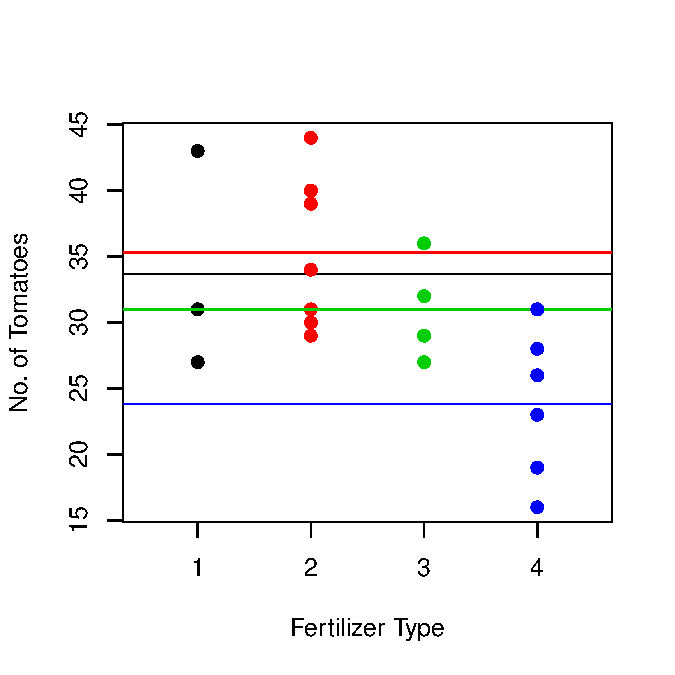
\includegraphics{figure/lec22-004}
\end{center}
\end{frame}
%-------------------------------------------------------------------------------


%-------------------------------------------------------------------------------
\begin{frame}
\frametitle{Analysis of Variance}
%
% Comment this
%

%Say we have $k$ groups and want to compare the $k$ means:
%\[
%\mu_1, \mu_2, \ldots, \mu_k
%\]
%
%\pause \vspace{0.25cm}
%
%We could do ${k \choose 2}$ individual two-sample tests.\\
%\pause \vspace{0.25cm}
%
%Ex. for groups 1 \& 2:
%\begin{eqnarray*}
%H_0: && \mu_1 = \mu_2\\
%\mbox{vs. } H_a:  && \mu_1 \neq \mu_2
%\end{eqnarray*}
%\end{frame}
%%-------------------------------------------------------------------------------
%
%
%
%%-------------------------------------------------------------------------------
%\begin{frame}
%\frametitle{Analysis of Variance}
%%
%% Comment this
%%
%
%Or we do \blue{a single overall test} via \blue{Analysis of Variance ANOVA}:
%
%\vspace{0.5cm}
%
%\pause The hypothesis test is:
%\begin{eqnarray*}
%H_0: && \mu_1 = \mu_2 = \ldots = \mu_k\\
%\mbox{vs. } H_a:  && \mbox{at least one of the $\mu_i$'s are different}\\
%\end{eqnarray*}
%
%\end{frame}
%%-------------------------------------------------------------------------------
%
%
%
%%-------------------------------------------------------------------------------
%\begin{frame}
%\frametitle{Analysis of Variance}
%%
%% Comment this
%%
%
%ANOVA asks:  where is the overall variability of the observations originate from?
%
%\vspace{0.5cm}
%
%\pause The \blue{test statistic} used to compute a $p$-value is now the \blue{F-statistic}:
%\[
%F = \frac{\mbox{measure of between-group variability}}{\mbox{measure of within-group variability}}
%\]

\end{frame}
%-------------------------------------------------------------------------------


%-------------------------------------------------------------------------------
\begin{frame}
\frametitle{Tomato Fertilizer Example}
Numerator: the \blue{between-group variation} refers to the variability \blue{between} the levels (the 4 horizontal lines):  
\setkeys{Gin}{width=0.65\textwidth}
\begin{center}
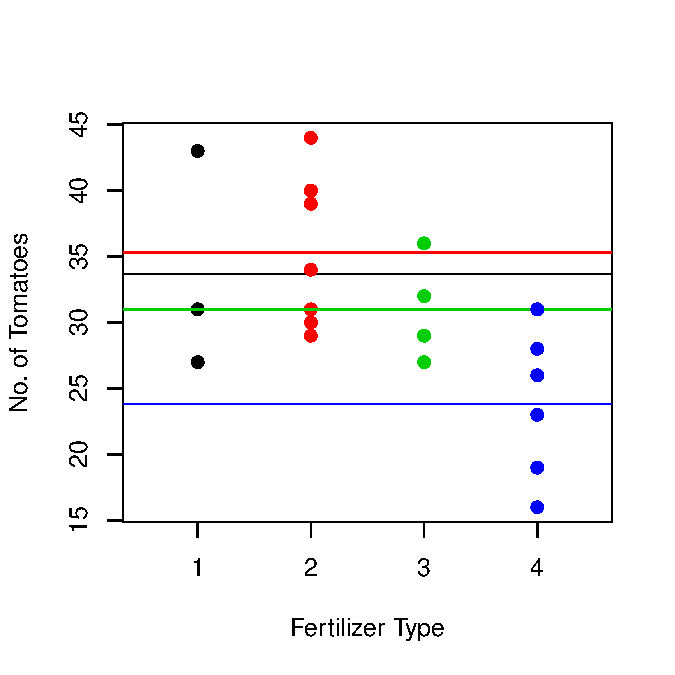
\includegraphics{figure/lec22-006}
\end{center}
\end{frame}
%-------------------------------------------------------------------------------


%-------------------------------------------------------------------------------
\begin{frame}
\frametitle{Tomato Fertilizer Example}
Denominator: the \blue{within-group variation} refers to the variability \blue{within} each level (the 4 vertical arrows):
\setkeys{Gin}{width=0.65\textwidth}
\begin{center}
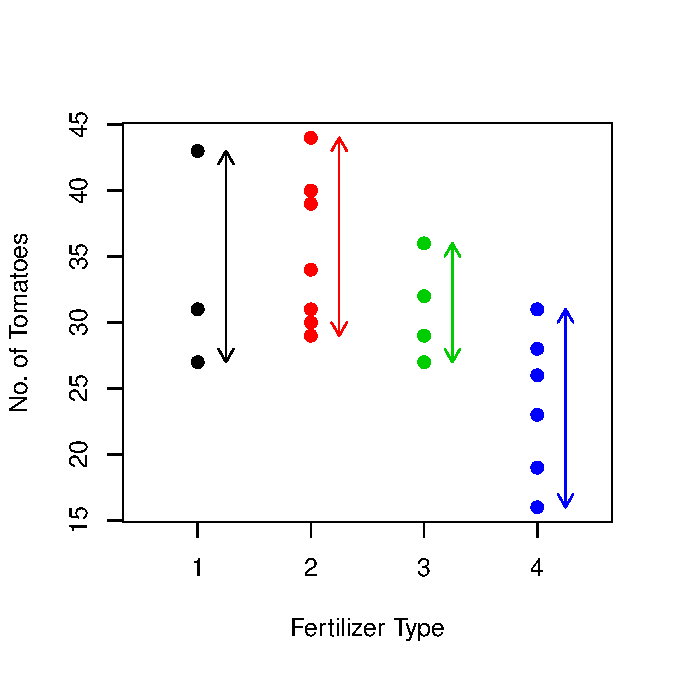
\includegraphics{figure/lec22-005}
\end{center}
\end{frame}
%-------------------------------------------------------------------------------


%-------------------------------------------------------------------------------
\begin{frame}
\frametitle{Tomato Fertilizer Example}
Now compare the following two plots.  Which has ``more different'' means?
\setkeys{Gin}{width=0.8\textwidth}
\begin{center}
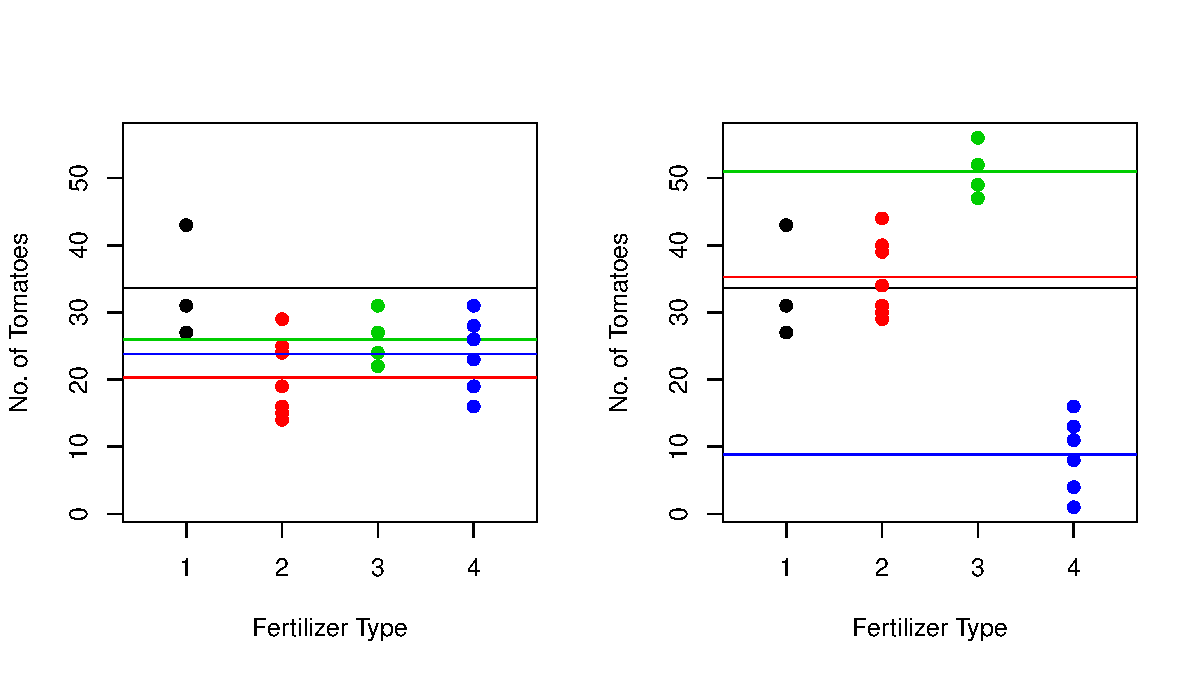
\includegraphics{figure/lec22-008}
\end{center}

\end{frame}
%-------------------------------------------------------------------------------


%-------------------------------------------------------------------------------
\begin{frame}
\frametitle{Tomato Fertilizer Example}

%
% Comment this
%
%\begin{itemize}
%\item They have the \blue{same within-group} variability.  Call this value $W$
%\pause \item The right plot has \blue{higher between group variability}  b/c the 4 means are more different.  Call these values $B_{left}$ and $B_{right}$ with $B_{left} < B_{right}$
%\pause \item Recall $F = \frac{\mbox{measure of between-group variability}}{\mbox{measure of within-group variability}}$
%\pause \item Since $\frac{B_{left}}{W} < \frac{B_{right}}{W}$, thus $F_{left} < F_{right}$
%\pause The right plot as a larger $F$-statistic
%\end{itemize}

\end{frame}
%-------------------------------------------------------------------------------


%-------------------------------------------------------------------------------
\begin{frame}
\frametitle{$F$ Distributions}
%
% Comment this
%
%\blue{Assuming $H_0$ is true} (that $\mu_1 = \mu_2 = \ldots = \mu_k$), the $F$-statistic
%\[
%F = \frac{\mbox{measure of between-group variability}}{\mbox{measure of within-group variability}}
%\]
%follows the \blue{$F$ distribution with $df_1=k-1$ and $df_2=n-k$ degrees of freedom } where
%\begin{itemize}
%\pause \item $n$ = \blue{total} number of observations
%\item $k$ = number of groups
%\end{itemize}
 
\end{frame}
%-------------------------------------------------------------------------------


%-------------------------------------------------------------------------------
\begin{frame}
\frametitle{$F$ Distributions}
For $df_1 = 4$ and $df_2=6$, the $F$ distribution looks like:
\setkeys{Gin}{width=0.65\textwidth}
\begin{center}
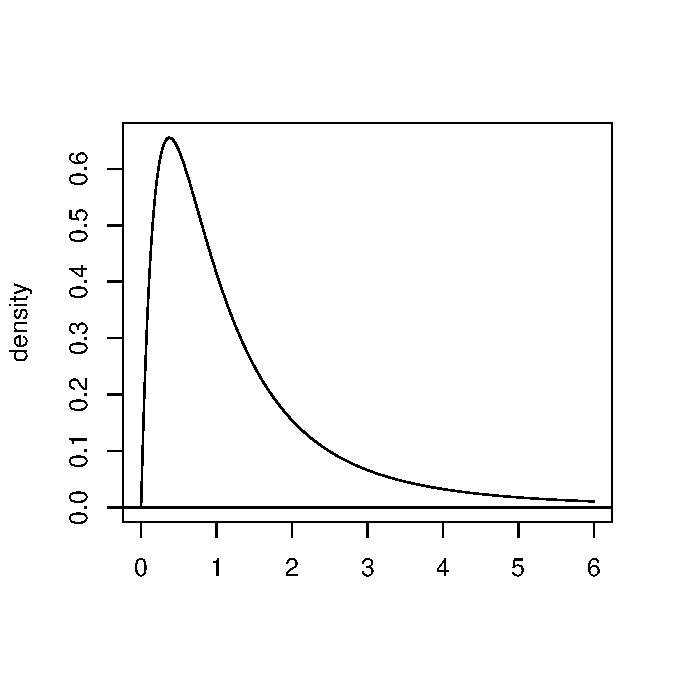
\includegraphics{figure/lec22-009}
\end{center}
\end{frame}
%-------------------------------------------------------------------------------


%-------------------------------------------------------------------------------
\begin{frame}
\frametitle{$F$ Distributions}
$p$-values are computed where ``more extreme'' means \blue{larger}.  Say the $F=3$, the $p$-value is the \blue{area to the right of 3}. %and is computed in {\tt R}: {\tt pf(3,df1=4,df2=6,lower.tail=FALSE)}
\setkeys{Gin}{width=0.65\textwidth}
\begin{center}
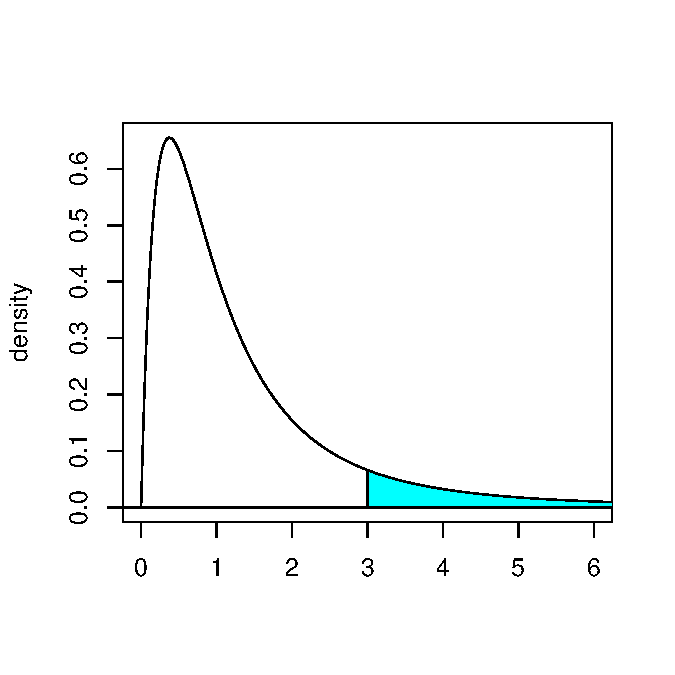
\includegraphics{figure/lec22-010}
\end{center}
\end{frame}
%-------------------------------------------------------------------------------


%-------------------------------------------------------------------------------
\begin{frame}
\frametitle{Conducting An $F$-Test}
The results are typically summarized in an \blue{ANOVA table}:

\begin{small}
\begin{center}
\begin{tabular}{l|ccc|cc}
Source of Variation & $df$ & $SS$ & $MS$ & $F$ & $p$-value\\
\hline
Between groups & $k-1$ & $SSTr$ & $MSTr = \frac{SSTr}{k-1}$ & $\frac{MSTr}{MSE}$ & $p$\\
Within groups & $n-k$ & $SSE$ & $MSE = \frac{SSE}{n-k}$ & & \\
\hline
Total & $n-1$ & $SST$ &  & & 
\end{tabular}
\end{center}
\end{small}
\end{frame}
%-------------------------------------------------------------------------------


%-------------------------------------------------------------------------------
\begin{frame}
\frametitle{Conditions}

\begin{enumerate}
\item The observations have to be \blue{independent}.  10\% rule.  
\pause \item Trade off of $n$ and \blue{normality} of observations \blue{within each group}. 
\pause \item Each of the groups has \blue{constant variance} $\sigma_1^2 = \ldots = \sigma_k^2 = \sigma^2$.  Check via:
\begin{itemize}
\item boxplots
\item comparing the sample standard deviations $s_1, \ldots, s_k$
\end{itemize}
\end{enumerate}

\end{frame}
%-------------------------------------------------------------------------------




\end{document}


























% Made this a HW question:


%------------------------------------------------------------------------------
\begin{frame}[fragile]
\frametitle{Multiple Testing}
You conduct $n=20$ tests of different jelly beans colors at the $\alpha=0.05$ significance level.  We expect 5\% of them to be significant by chance alone.  

\pause \vspace{0.5cm}

If the tests are independent, the number of significant tests is \blue{Binomial}$(n=20, p=\alpha=0.05)$.  

\pause \vspace{0.5cm}

We saw in Chapter 3 
\[\mu = np = 20 \times 0.05 = 1 \mbox{ test}\]

\end{frame}
%------------------------------------------------------------------------------


%------------------------------------------------------------------------------
\begin{frame}[fragile]
\frametitle{Multiple Testing}
What is
\begin{eqnarray*}
P(\mbox{at least one sig result in 20}) &=& \pause 1 - P(\mbox{no sig results in 20})\\
\pause &=& 1 - {20 \choose 0} \alpha^{0} (1-\alpha)^{20} \\
\pause &=& 1- (1-0.05)^{20}\\
\pause &\approx& 0.64
\end{eqnarray*}

\pause We have 64\% chance of observing at least one significant result, even if ``nothing is going on.''

\vspace{0.25cm}

\pause Why?  Because we did so many tests!  That is a huge chance of a false positive!
\end{frame}
%------------------------------------------------------------------------------


%------------------------------------------------------------------------------
\begin{frame}[fragile]
\frametitle{Multiple Testing}
So in our case, use $\alpha^* = \frac{0.05}{20} = 0.0025$.  \pause Now
\begin{eqnarray*}
P(\mbox{at least one sig result in 20}) &=& \pause 1 - P(\mbox{no sig results in 20})\\
&=& 1 - {20 \choose 0} \alpha^{*0} (1-\alpha^{*})^{20} \\
&=& 1- (1-0.0025)^{20}\\
&\approx& 0.0488
\end{eqnarray*}

\pause Closer to \blue{true desired} $\alpha=0.05$.  

\vspace{0.25cm}

\pause \blue{Note}: the correction is conservative in that the overall type I error rate is $0.0488 < 0.05$.

\end{frame}
%------------------------------------------------------------------------------










